\begin{figure}[ht]
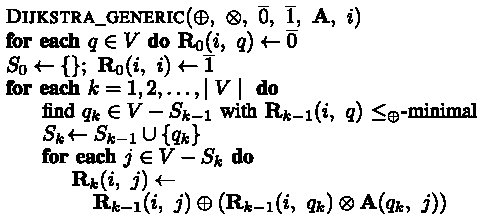
\includegraphics{algorithm.pdf}
\caption{Dynerowicz and Griffin's imperative generalised Dijkstra's algorithm}
\label{fig.algorithm}
\end{figure}

Given a weighted graph $G$, Dijkstra's algorithm in its standard form finds the shortest distance from some start node $i \in G$ to each other connected node $j \in G$, provided all edges in $G$ have non-negative weight.
Dynerowicz and Griffin~\cite{dynerowicz_forwarding_2013} found that a generalised variant of Dijkstra's algorithm finds one row of the matrix $R$ solving the fixpoint equation:
\begin{displaymath}
R = I + (R \times A)
\end{displaymath}
Here, $A$ is the adjacency matrix of the graph $G$ and $I$ the identity matrix.
All matrix coefficients are taken from the carrier set of a Sobrinho Algebra, with $-+-$ and $-\times-$ the binary addition and multiplication operations of a Sobrinho Algebra lifted to matrices (see Section~\ref{sect.path.algebras.their.properties.and.models}).
Pseudocode for the imperative generalised Dijkstra algorithm, as presented by Dynerowicz and Griffin~\cite[pg. 9]{dynerowicz_forwarding_2013}, is provided in Figure~\ref{fig.algorithm}.

\todo{finish this description}
